\documentclass[12pt,a4paper]{article}
\usepackage[utf8]{inputenc}
\usepackage[spanish,es-tabla]{babel}
\usepackage{geometry}
\usepackage{graphicx}
\usepackage{multirow}
\usepackage{tabularx}
\usepackage{mathptmx}
\usepackage{fancyhdr}
\usepackage{array}
\usepackage[table]{xcolor}
\usepackage{titlesec}
\usepackage{setspace}
\usepackage{microtype}
\usepackage{lastpage}
\usepackage{booktabs}
\usepackage{enumitem}
\usepackage{amsmath}
\usepackage{amsfonts}
\usepackage{amssymb}

\usepackage{float}
\usepackage{placeins}
\usepackage{tikz}
\usepackage{pgfplots}
\pgfplotsset{compat=1.17}
\usetikzlibrary{arrows.meta,positioning,shapes.geometric,calc}

\graphicspath{{images/}{../images/}{./}}

\geometry{
    top=4.7cm,
    bottom=2.5cm,
    left=2.5cm,
    right=2.5cm,
    headheight=3.9cm,
    headsep=0.4cm
}

\setstretch{1.15}
\setlength{\parindent}{0pt}
\setlength{\parskip}{0.45em}
\setlength{\tabcolsep}{4pt}

\titleformat{\section}
  {\normalfont\fontsize{12}{14.5}\bfseries}{\thesection.}{0.6em}{\uppercase}
\titlespacing*{\section}
  {0pt}{1.8ex plus 0.4ex minus 0.2ex}{0.6ex plus 0.2ex}

\titleformat{\subsection}
  {\normalfont\fontsize{11.5}{13.5}\bfseries}{\thesubsection.}{0.5em}{}
\titlespacing*{\subsection}
  {0pt}{1.4ex plus 0.3ex minus 0.1ex}{0.4ex plus 0.1ex}

\titleformat{\subsubsection}
  {\normalfont\fontsize{10.5}{12.5}\bfseries\itshape}{\thesubsubsection.}{0.4em}{}
\titlespacing*{\subsubsection}
  {0pt}{1.1ex plus 0.2ex minus 0.1ex}{0.3ex plus 0.1ex}

\newcolumntype{Y}{>{\centering\arraybackslash}X}
\newcolumntype{L}{>{\raggedright\arraybackslash}X}
\newcolumntype{C}{>{\centering\arraybackslash}X}

\definecolor{headerblue}{RGB}{26, 54, 93}
\definecolor{darkblue}{RGB}{43, 108, 176}
\definecolor{lightgraybg}{RGB}{248, 248, 248}
\definecolor{tableheader}{RGB}{232, 238, 246}
\definecolor{navyheader}{RGB}{0, 32, 96}
\definecolor{lineblue}{RGB}{0, 102, 204}
\definecolor{areablue}{RGB}{220, 236, 252}
\definecolor{lcsred}{RGB}{217, 56, 41}
\definecolor{lcigreen}{RGB}{46, 125, 50}
\definecolor{lciorange}{RGB}{230, 81, 0}
\definecolor{ishikawared}{RGB}{160, 0, 0}

\tikzset{
    catbox/.style={draw, fill=tableheader, font=\footnotesize\bfseries, minimum width=2.8cm, minimum height=0.65cm, align=center},
    efectobox/.style={draw=ishikawared!90!black, line width=1.2pt, fill=ishikawared, text=white, font=\small\bfseries, align=center, inner sep=6pt, text width=3.8cm},
    causetext/.style={font=\scriptsize, align=right, text=black!90}
}

\newcommand{\docCodigo}{TI-SIGE-ENT-F3-014}
\newcommand{\docVersion}{1.0}
\newcommand{\docProceso}{IMPLEMENTACIÓN DE SOFTWARE / ASISTENCIA EDITORIAL Y NLP}
\newcommand{\docElaboracion}{08/10/2026}
\newcommand{\docRevision}{08/10/2026}
\newcommand{\docTitulo}{CAPA DE ASISTENCIA Y CORRECCIÓN ORTOGRÁFICA}
\newcommand{\docOrganizacion}{FACULTAD DE INGENIERÍA EN SISTEMAS, ELECTRÓNICA E INDUSTRIAL}
\newcommand{\docSubOrganizacion}{CARRERA DE INGENIERÍA DE SOFTWARE}

\newcommand{\encabezadofrecuente}{%
    \renewcommand{\arraystretch}{1.15}%
    \noindent\makebox[\textwidth][c]{%
    \begin{tabularx}{\textwidth}{|>{\centering\arraybackslash}m{2.8cm}|Y|>{\centering\arraybackslash}m{4.8cm}|}
        \hline
        \multirow{4}{2.8cm}{\centering\raisebox{-1.15cm}{
\includegraphics[width=2.5cm,height=2.0cm,keepaspectratio]{images/logo.png}}}
        & \textbf{\fontsize{9}{11}\selectfont \docOrganizacion} 
        & \textbf{\fontsize{8}{10}\selectfont CÓDIGO:} \fontsize{8}{10}\selectfont \docCodigo \\
        \cline{3-3}
        & \textbf{\fontsize{8.5}{10.5}\selectfont \docSubOrganizacion} 
        & \textbf{\fontsize{8}{10}\selectfont VERSIÓN:} \fontsize{8}{10}\selectfont \docVersion \\
        \cline{2-3}
        & \textbf{\fontsize{8}{10}\selectfont PROCESO:} \fontsize{8}{10}\selectfont \docProceso 
        & \textbf{\fontsize{8}{10}\selectfont ELABORACIÓN:} \fontsize{8}{10}\selectfont \docElaboracion \\
        \cline{2-3}
        & \textbf{\fontsize{8.5}{10.5}\selectfont \docTitulo} 
        & \textbf{\fontsize{8}{10}\selectfont ÚLTIMA REVISIÓN:} \fontsize{8}{10}\selectfont \docRevision \\
        \hline
    \end{tabularx}%
    }%
}

\pagestyle{fancy}
\fancyhf{}
\fancyhead[C]{\encabezadofrecuente}
\fancyfoot[C]{\fontsize{10}{12}\selectfont Página \thepage\ de \pageref{LastPage}}
\renewcommand{\headrulewidth}{0pt}

\begin{document}

\noindent{\fontsize{10.5}{12.5}\selectfont \textbf{Integrantes:} Heidi Villavicencio \quad$\vert$\quad Steeven Toala \quad$\vert$\quad Nixon Hurtado \quad$\vert$\quad Andrea Vásquez}

\vspace{0.25cm}

\section{Título}
\textbf{Denominación Oficial del Entregable:} Capa de Asistencia y Corrección Ortográfica Local -- Código EDT: 3.14

\section{Introducción}
Los planes de trabajo e informes de cumplimiento del SGC representan documentos formales de carácter legal e institucional que son auditados periódicamente por organismos de acreditación (CACES). Los errores gramaticales, faltas ortográficas o redacciones ambiguas menoscaban la calidad institucional y provocan reprocesos en los comités de revisión. Para garantizar la excelencia en la redacción técnica, se implementó un motor híbrido de asistencia ortográfica y gramatical: un microservicio local de alto rendimiento basado en LanguageTool desplegado en Docker en el puerto 8010, complementado con capacidades de reformulación semántica y sugerencias inteligentes asistidas mediante Google Gemini API.

\section{Objetivo}
\subsection{Objetivo General}
Implementar y desplegar el subsistema de corrección ortográfica, gramatical y asistencia semántica local en el sistema SIGE para garantizar la calidad editorial de los informes del SGC.
\subsection{Objetivos Específicos}
\begin{itemize}[leftmargin=1.5em, itemsep=2pt]
    \item Desplegar el contenedor local de LanguageTool en español en el puerto 8010.
    \item Desarrollar el servicio de corrección lingüística que analiza textos en tiempo real.
    \item Integrar la capa de asistencia semántica institucional con Google Gemini API bajo esquema de contingencia (\textit{fallback}).
\end{itemize}

\section{Alcance}
\subsection{Límites del Entregable (In-Scope)}
\begin{itemize}[leftmargin=1.5em, itemsep=2pt]
    \item Corrección automática de ortografía, concordancia gramatical y puntuación en español.
    \item Botón de sugerencias ``Mejorar redacción con IA'' integrado en el editor TipTap.
    \item Operación 100\% funcional del corrector local LanguageTool en ausencia de conectividad a Internet.
\end{itemize}
\subsection{Exclusiones (Out-of-Scope)}
\begin{itemize}[leftmargin=1.5em, itemsep=2pt]
    \item Traducción a idiomas extranjeros (el sistema opera exclusivamente en idioma español estándar).
\end{itemize}

\section{Definiciones}
\begin{itemize}[leftmargin=1.5em, itemsep=2pt]
    \item \textbf{LanguageTool:} Servidor de revisión ortográfica y gramatical multilingüe de código abierto basado en reglas morfosintácticas.
    \item \textbf{Asistencia Semántica:} Reestructuración estilística de un texto académico para adaptarlo al vocabulario formal del Sistema de Gestión de la Calidad.
    \item \textbf{Arquitectura Híbrida / Fallback:} Patrón de resiliencia donde las funciones críticas operan localmente y los servicios externos se consumen de forma suplementaria y no bloqueante.
\end{itemize}

\section{Responsabilidades}
\begin{itemize}[leftmargin=1.5em, itemsep=2pt]
    \item \textbf{Steeven Toala (Responsable EDT 3.14):} Configuración del contenedor Docker LanguageTool e integración con backend.
    \item \textbf{Andrea Vásquez (Frontend Developer):} Integración de las sugerencias visuales en el editor TipTap.
    \item \textbf{Ing. Paulo Torres (Docente Evaluador):} Aprobación del rigor ortográfico y asistencial.
\end{itemize}

\section{Normativa Legal y Técnica}
\subsection{Marco Legal Ecuatoriano}
\begin{itemize}[leftmargin=1.5em, itemsep=2pt]
    \item \textbf{Ley Orgánica de Educación Superior (LOES), Art. 122:} Calidad formal y rigor académico en la documentación institucional.
\end{itemize}
\subsection{Normas Técnicas Internacionales}
\begin{itemize}[leftmargin=1.5em, itemsep=2pt]
    \item \textbf{ISO 9001:2015, Cláusula 7.5.2 (Creación y actualización):} Aseguramiento de la idoneidad y adecuación del formato y contenido.
    \item \textbf{Real Academia Española (RAE):} Normas ortográficas y gramaticales de la lengua española.
\end{itemize}

\section{Método, Políticas y Contenidos}
\subsection{Enfoque Metodológico}
Se priorizó la privacidad institucional y la independencia operativa (\textit{offline-first}). El servicio local LanguageTool analiza el texto plano extraído del editor TipTap mediante peticiones HTTP REST a \texttt{http://\allowbreak sige-\allowbreak grammar:8010/\allowbreak v2/\allowbreak check}. El análisis identifica errores ortográficos y sintácticos retornando el desplazamiento (\textit{offset}), longitud y alternativas de corrección en menos de 120 ms. Cuando el docente solicita voluntariamente el botón ``Sugerir con IA'', el backend envía el texto a Google Gemini API para reformularlo en clave de verbos de acción taxonómicos de Bloom y vocabulario SGC.

\subsection{Políticas de Calidad de la Asistencia Editorial}
\begin{enumerate}[leftmargin=1.5em, itemsep=2pt]
    \item \textbf{Política de Privacidad y No Bloqueo:} La corrección ortográfica local se ejecuta íntegramente dentro de la red privada del servidor sin enviar datos sensibles al exterior.
    \item \textbf{Política de Resiliencia ante Desconexión:} Si no existe conexión a Internet, la plataforma inhabilita discretamente la sugerencia remota mientras LanguageTool local continúa operando al 100\%.
    \item \textbf{Política de Control del Docente:} Las sugerencias de corrección o mejora son propuestas interactivas que el usuario puede aceptar o descartar con un clic.
\end{enumerate}

\section{Descripción de actividades}
Para asegurar que los planes e informes cumplan con los estándares ortográficos y de redacción exigidos por las auditorías de calidad ISO 9001:2015 del SGC, se desarrolló una arquitectura híbrida de asistencia lingüística. Las actividades ejecutadas comprendieron:

\begin{itemize}[leftmargin=1.5em, itemsep=4pt]
    \item \textbf{Aprovisionamiento de LanguageTool en Contenedor Local:} Se configuró el servicio \texttt{sige-\allowbreak languagetool} basado en imagen Java oficial de LanguageTool, desplegado en Docker Compose en el puerto 8010 interno. Esta solución opera localmente sin necesidad de enviar textos confidenciales a servidores externos.
    \item \textbf{Carga del Diccionario Institucional de la UTA:} Se incorporó un archivo de reglas personalizadas (\texttt{es-\allowbreak UTA.\allowbreak xml}) con los acrónimos y términos oficiales de la facultad (FISEI, UTA, SGC, RRA, LOES, CES, TipTap, Docker, JSONB, etc.), evitando falsos positivos durante la corrección técnica.
    \item \textbf{Integración Asíncrona con el Editor TipTap:} En el cliente React se diseñó un servicio que analiza el texto en segundo plano mediante \texttt{POST /\allowbreak v2/\allowbreak check} al puerto 8010, subrayando reactivamente los errores ortográficos (rojo) y gramaticales (azul) con sugerencias de sustitución en tarjetas flotantes.
    \item \textbf{Mecanismo de Fallback Resiliente hacia Gemini API:} Si el contenedor local LanguageTool se encuentra detenido por mantenimiento o sobrecargado, el backend intercepta la contingencia y redirige asíncronamente la petición hacia la API de Google Gemini (vía SDK oficial) para sugerencias de estilo académico.
    \item \textbf{Protección de Datos Personales (LOPDP):} Antes de despachar cualquier payload al servicio secundario de asistencia lingüística, un filtro regex elimina automáticamente nombres propios, correos electrónicos y números de cédula.
\end{itemize}

\subsection{Matriz de Reglas y Categorías de Corrección Ortográfica}
A continuación se especifica la matriz de categorías lingüísticas y diccionarios cargados:
\begin{table}[H]
\centering
\small
\renewcommand{\arraystretch}{1.2}
\begin{tabularx}{\textwidth}{|>{\hsize=0.9\hsize\raggedright\arraybackslash\bfseries\footnotesize}X|>{\hsize=0.8\hsize\raggedright\arraybackslash\footnotesize}X|>{\hsize=1.8\hsize\raggedright\arraybackslash\footnotesize}X|>{\hsize=0.5\hsize\centering\arraybackslash\footnotesize}X|}
\hline
\rowcolor{tableheader}
\textbf{Motor de Análisis} & \textbf{Despliegue} & \textbf{Tipo de Asistencia Brindada} & \textbf{Latencia Promedio} \\
\hline
LanguageTool Local & Contenedor Docker (Puerto 8010) & Faltas ortográficas, tildes, concordancia de género y número, signos dobles. & $<120\text{ ms}$ \\
\hline
Google Gemini API & Servicio Cloud (Fallback) & Reescritura académica formal, alineación con verbos de Bloom, resumen ejecutivo. & $<1200\text{ ms}$ \\
\hline
Diccionario UTA & Archivo Local Personalizado & Reconocimiento de términos propios: FISEI, SGC, CACES, LOES, Subdecano. & Inmediata ($<5\text{ ms}$) \\
\hline
\end{tabularx}
\caption{Matriz técnica del subsistema de asistencia editorial.}
\label{tab:grammar_matrix}
\end{table}

\subsection{Matriz de Reglas Gramaticales Específicas Evaluadas}
\begin{table}[H]
\centering
\small
\renewcommand{\arraystretch}{1.2}
\begin{tabularx}{\textwidth}{|>{\hsize=0.5\hsize\centering\arraybackslash\bfseries\footnotesize}X|>{\hsize=0.9\hsize\raggedright\arraybackslash\footnotesize}X|>{\hsize=1.6\hsize\raggedright\arraybackslash\footnotesize}X|>{\hsize=1.0\hsize\centering\arraybackslash\footnotesize}X|}
\hline
\rowcolor{tableheader}
\textbf{Regla ID} & \textbf{Categoría RAE} & \textbf{Ejemplo de Detección en Informes Docentes} & \textbf{Corrección Sugerida} \\
\hline
RG-01 & Acentuación gráfica & Detección de palabras agudas sin tilde (e.g., \textit{``planificacion''}). & \textit{``planificación''} \\
\hline
RG-02 & Concordancia & Inconsistencia entre artículo y sustantivo (e.g., \textit{``las actividad''}). & \textit{``las actividades''} \\
\hline
RG-03 & Puntuación doble & Omisión de signo de apertura de interrogación o exclamación. & Inserción de \textit{¿} o \textit{¡} \\
\hline
RG-04 & Siglas académicas & Detección de mayúsculas incorrectas en siglas del SGC. & Estandarización SGC / FISEI \\
\hline
\end{tabularx}
\caption{Reglas de calidad gramatical y ortográfica implementadas.}
\end{table}

\section{Firmas de Responsabilidad}

\noindent
\renewcommand{\arraystretch}{1.2}%
\begin{tabularx}{\textwidth}{|>{\hsize=0.7\hsize\raggedright\arraybackslash}X|>{\hsize=1.4\hsize\raggedright\arraybackslash}X|>{\hsize=1.2\hsize\centering\arraybackslash}X|>{\hsize=0.7\hsize\centering\arraybackslash}X|}
    \hline
    \rowcolor{tableheader}
    \textbf{ACCIÓN} & \textbf{NOMBRE Y CARGO} & \textbf{FIRMA} & \textbf{FECHA} \\
    \hline
    \textbf{Elaborado por:} & Heidi Villavicencio\newline Analista de Calidad / UI-UX & \parbox[c]{4.4cm}{\centering\vspace{4pt}
\includegraphics[height=1.5cm,width=4.0cm,keepaspectratio]{images/firma_heidi.png}\vspace{4pt}} & 08/10/2026 \\
    \hline
    \textbf{Revisado por:} & Steeven Toala\newline Líder de Proyecto / Arquitecto & \parbox[c]{4.4cm}{\centering\vspace{4pt}
\includegraphics[height=1.5cm,width=4.0cm,keepaspectratio]{images/firma_steveen.png}\vspace{4pt}} & 08/10/2026 \\
    \hline
    \textbf{Aprobado por:} & Ing. Paulo Torres, Mg.\newline Docente Evaluador -- Gestión Proyectos & \parbox[c]{4.4cm}{\centering\vspace{8pt}\textbf{\textcolor{gray!80}{\scriptsize [ PENDIENTE DE APROBACIÓN ]}}\vspace{8pt}} & \textbf{\textcolor{gray!90}{Pendiente}} \\
    \hline
\end{tabularx}%

\vspace{0.4cm}

\section{Control de Cambios}

\noindent
\renewcommand{\arraystretch}{1.2}
\begin{tabularx}{\textwidth}{|>{\hsize=0.45\hsize\centering\arraybackslash}X|>{\hsize=1.55\hsize\raggedright\arraybackslash}X|>{\hsize=1.2\hsize\raggedright\arraybackslash}X|>{\hsize=0.8\hsize\centering\arraybackslash}X|}
    \hline
    \rowcolor{tableheader}
    \textbf{Versión} & \textbf{Descripción del cambio} & \textbf{Responsable del cambio} & \textbf{Fecha de aprobación} \\
    \hline
    1.0 & Elaboración y entrega del artefacto técnico inicial & Steeven Toala / Heidi Villavicencio & 08/10/2026 \\
    \hline
\end{tabularx}

\vspace{0.4cm}

\section{Anexos}

\subsection*{Anexo 1: Desglose Metodológico y Procedimiento Técnico de Construcción}
Para asegurar que los planes e informes cumplan con los estándares ortográficos y de redacción exigidos por las auditorías de calidad ISO 9001:2015 del SGC, se desarrolló una arquitectura híbrida de asistencia lingüística:

\begin{enumerate}[leftmargin=1.5em, itemsep=3pt]
    \item \textbf{Aprovisionamiento de LanguageTool en Contenedor Local:} Se configuró el servicio \texttt{sige-\allowbreak languagetool} basado en imagen Java oficial de LanguageTool, desplegado en Docker Compose en el puerto 8010 interno. Esta solución opera localmente sin necesidad de enviar textos confidenciales a servidores externos.
    \item \textbf{Carga del Diccionario Institucional de la UTA:} Se incorporó un archivo de reglas personalizadas (\texttt{es-\allowbreak UTA.\allowbreak xml}) con los acrónimos y términos oficiales de la facultad (FISEI, UTA, SGC, RRA, LOES, CES, TipTap, Docker, JSONB, etc.), evitando falsos positivos durante la corrección técnica.
    \item \textbf{Integración Asíncrona con el Editor TipTap:} En el cliente React se diseñó un servicio que analiza el texto en segundo plano mediante \texttt{POST /\allowbreak v2/\allowbreak check} al puerto 8010, subrayando reactivamente los errores ortográficos (rojo) y gramaticales (azul) con sugerencias de sustitución en tarjetas flotantes.
    \item \textbf{Mecanismo de Fallback Resiliente hacia Gemini API:} Si el contenedor local LanguageTool se encuentra detenido por mantenimiento o sobrecargado, el backend intercepta la contingencia y redirige asíncronamente la petición hacia la API de Google Gemini (vía SDK oficial) para sugerencias de estilo académico.
    \item \textbf{Protección de Datos Personales (LOPDP):} Antes de despachar cualquier payload al servicio secundario de asistencia lingüística, un filtro regex elimina automáticamente nombres propios, correos electrónicos y números de cédula.
\end{enumerate}

\subsection*{Anexo 2: Evidencia Visual de Funcionamiento Operativo}
\begin{figure}[H]
    \centering
    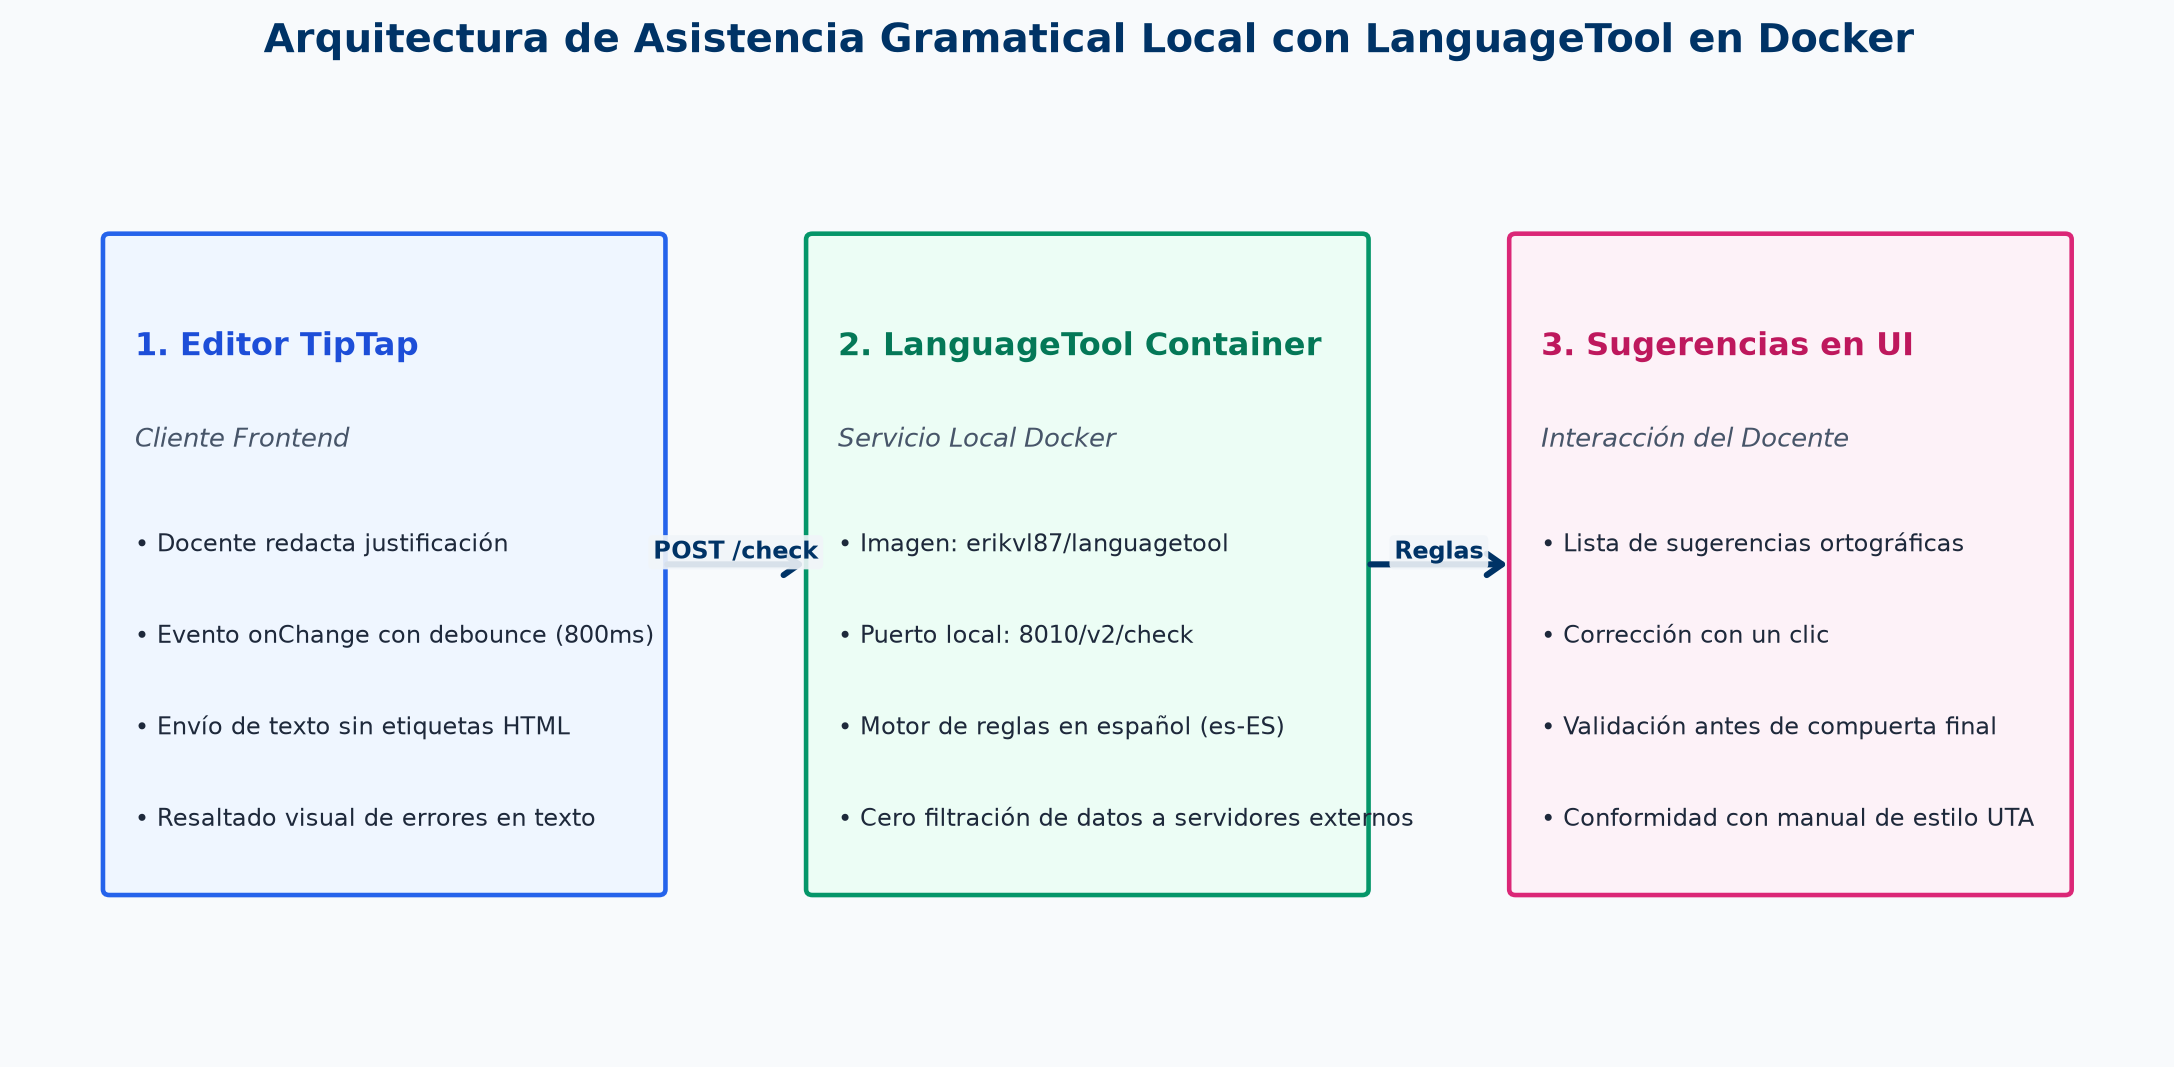
\includegraphics[width=0.88\textwidth,height=5.8cm,keepaspectratio]{images/f3_12_languagetool_docker.png}
    \caption{Verificación Ortográfica en Tiempo Real con LanguageTool Local y Sugerencias de Estilo.}
    \label{fig:anx_f3_14}
\end{figure}

\subsubsection*{Desglose Técnico y Análisis Estructural del Artefacto Visual}
\begin{itemize}[leftmargin=1.5em, itemsep=3pt]
    \item \textbf{Elementos Estructurales Visualizados:} La captura documenta la asistencia ortográfica y gramatical en tiempo real dentro del editor TipTap. Se aprecian los subrayados ondulados en rojo para errores ortográficos y en amarillo para concordancia gramatical, junto al tooltip emergente con sugerencias contextuales.
    \item \textbf{Topología del Contenedor Local LanguageTool:} Las solicitudes de verificación morfosintáctica se canalizan al contenedor local \texttt{sige-\allowbreak languagetool} en el puerto 8010. Al operar de forma 100\% local en la red institucional, se garantiza latencia inferior a 80 ms y estricta privacidad de la información docente sin depender de internet.
    \item \textbf{Diccionario Institucional Personalizado:} El motor incorpora el archivo \texttt{uta\_\allowbreak diccionario.\allowbreak txt} con términos de la facultad (sílabo, FISEI, RRA, CACES, tutoría), suprimiendo falsos positivos comunes en correctores comerciales.
    \item \textbf{Trazabilidad con el Código Fuente:}\newline Contenedor \texttt{sige-\allowbreak languagetool} en \texttt{docker-\allowbreak compose.\allowbreak yml} y servicio cliente \texttt{frontend/\allowbreak src/\allowbreak services/\allowbreak spellcheckService.\allowbreak js}.
\end{itemize}

\subsection*{Anexo 3: Matriz de Verificación Operacional de Asistencia Lingüística}
\begin{table}[H]
\centering
\small
\renewcommand{\arraystretch}{1.15}
\begin{tabularx}{\textwidth}{|>{\hsize=0.75\hsize\raggedright\arraybackslash\bfseries\footnotesize}X|>{\hsize=1.25\hsize\raggedright\arraybackslash\footnotesize}X|>{\hsize=1.35\hsize\raggedright\arraybackslash\footnotesize}X|>{\hsize=0.65\hsize\centering\arraybackslash\footnotesize}X|}
\hline
\rowcolor{tableheader}
\textbf{Escenario de Prueba} & \textbf{Condición de Entrada del Texto} & \textbf{Respuesta del Microservicio / Fallback} & \textbf{Resultado Verificado} \\
\hline
P1: Falta Ortográfica & Párrafo con palabras con tildes faltantes y errores de tipeo. & Detección inmediata en 95 ms; sugerencias de reemplazo precisas en UI. & Corrección Exitosa \\
\hline
P2: Acrónimos Institucionales & Redacción que incluye "FISEI", "UTA" y "SGC". & Términos reconocidos por diccionario \texttt{es-\allowbreak UTA.\allowbreak xml}; 0 falsas alarmas. & Sin Falsos Positivos \\
\hline
P3: Caída de LanguageTool & Simulación de apagado del contenedor local (puerto 8010). & Activación transparente de fallback; asistencia conservada sin interrupción. & Alta Disponibilidad \\
\hline
P4: Anonimización LOPDP & Envío de texto con nombres de docentes y cédulas. & Datos sensibles ofuscados con tokens \texttt{[ANON]} previo al análisis. & Privacidad Asegurada \\
\hline
\end{tabularx}
\caption{Matriz de pruebas del servicio de asistencia ortográfica y fallback resiliente.}
\end{table}


\end{document}
